% Verification report for the wave-resistance solver.
% Prepared in the VOILAb paper-template style (Viola, VOILAb Paper-Writing Guide, 2025).
\documentclass[11pt]{article}

\usepackage[a4paper,margin=25mm]{geometry}
\usepackage{amsmath,amssymb,bm}
\usepackage{graphicx}
\usepackage{booktabs}
\usepackage{siunitx}
\usepackage{caption}
\usepackage[british]{babel}
\usepackage[hidelinks]{hyperref}
\usepackage{upgreek}
\usepackage{natbib}
\bibliographystyle{plainnat}

\sisetup{detect-all, per-mode=symbol, range-phrase={ to }, range-units=single}
\captionsetup{font=small, labelfont=bf}
\setlength{\parskip}{0pt}
\renewcommand{\arraystretch}{1.12}
\newcommand{\Fn}{\mathit{Fn}}

\title{\vspace{-12mm}\bfseries Wave Resistance of a Systematic Yacht Hull\\
by a Neumann--Kelvin Panel Method}
\author{}
\date{}

\begin{document}
\maketitle
\vspace{-16mm}

\begin{center}
\begin{minipage}{0.9\textwidth}
\small
\textbf{Verification report on the \texttt{wave-resistance} code.}\\[2mm]
Repository: \url{https://github.com/ignaziomviola/wave-resistance}\\
Commit reviewed: \texttt{ebbe169}\\
Report compiled: 21 August 2026
\end{minipage}
\end{center}

\vspace{4mm}
\begin{abstract}
\noindent
The \texttt{wave-resistance} code solves the Neumann--Kelvin problem for a bare
sailing-yacht canoe body by a constant-source panel method, with the Delft Systematic Yacht
Hull Series (DSYHS) hull Sysser 01 as the worked case. This report verifies the code
independently of its own assertions and reports the wave resistance across the measured
speed range. The implementation is correct at the level its analytic oracles can resolve:
its suite of 160 tests passes; the displaced volume computed by four independent
applications of the divergence theorem agrees to \num{3.0e-15}; the hydrostatics converge at
second order and match the published displaced volume and waterplane area to better than
\SI{0.06}{\percent}; and the Kelvin Green function satisfies the linearised free-surface
condition to \num{3.8e-08}, a property the code never imposes numerically. The wave resistance of
Sysser 01 is not converged on any mesh the code's throughput of
\SI{1164}{\micro\second} per panel pair permits. Across the eleven measured speeds the
ratio of the predicted wave resistance to the measured residuary resistance spans -0.46 to
+4.41 by the pressure route, and the predicted curve peaks at $\Fn = $~0.40 while the
measurement rises monotonically, so the agreement to 0.73 at $\Fn = 0.30$ is one point in
a wide scatter rather than a validation.
Two obstructions with disjoint speed ranges account for this and together cover the useful
range: below $\Fn \approx 0.35$ the measured residuary resistance is under
\SI{0.6}{\percent} of displacement weight, so the discretisation error is comparable to the
signal, while above $\Fn \approx 0.40$ the published data does not determine the running
attitude, the heave ambiguity from the unstated sinkage datum reaching
\SI{44}{\milli\metre} against a \SI{31}{\milli\metre} measured sinkage at $\Fn = 0.50$.
Two findings are added here: the stated worst-case accuracy of the wave-kernel gradient,
\num{7.0e-4}, holds at $\Fn = 0.30$ but is exceeded by a factor of four at $\Fn = 0.45$;
and the spectral cut-off can fall below the physical lower limit of the resistance integral
at low Froude number, where the code returns a resistance that is not meaningful without
flagging it as such.
\end{abstract}

\noindent\textbf{Key words:} wave resistance, Neumann--Kelvin problem, panel method,
Kelvin Green function, Delft Systematic Yacht Hull Series, code verification.

\section*{Nomenclature}
\noindent
\begin{tabular}{@{}ll@{\hspace{10mm}}ll@{}}
$a$      & Michell amplitude, nondimensional      & $\bm{n}$ & unit normal, into the fluid\\
$b$      & waterline beam                          & $p$      & pressure\\
$c$      & waterline length                        & $\bm{r}$ & position vector\\
$d$      & canoe-body draught                      & $u$      & speed of the onset flow\\
$\mathcal{G}$ & Kelvin Green function              & $\bm{u}$ & velocity, $(u,v,w)$\\
$g$      & gravitational acceleration              & $x,y,z$  & Cartesian coordinates\\
$\mathcal{A}$ & free-wave amplitude                & $\lambda$ & $\sec\theta$, wave parameter\\
$k_0$    & wavenumber scale, $g/u^2$               & $\theta$ & wave propagation angle\\
$W$      & displacement weight                     & $\rho$   & fluid density\\
$N$      & number of panels                        & $\sigma$ & source density\\
$R$      & resistance                              & $\phi$   & disturbance potential\\
$S$      & wetted surface                          & $\Phi$   & total potential\\
$\nabla_c$ & displaced volume of the canoe body    & $\Gamma$ & waterline, $S\cap\{z=0\}$\\
\end{tabular}

\vspace{3mm}
\noindent
\begin{tabular}{@{}ll@{}}
DSYHS & Delft Systematic Yacht Hull Series\\
IGES  & Initial Graphics Exchange Specification\\
ITTC  & International Towing Tank Conference\\
NURBS & Non-Uniform Rational B-Spline\\
$\Fn$ & Froude number, $u/\sqrt{gc}$\\
$Re$  & Reynolds number, $uc/\nu$\\
\end{tabular}

\section{Introduction}
Wave resistance is the part of a hull's resistance carried away by the free-surface
waves it generates, and for a sailing-yacht canoe body at a Froude number,
$\Fn \equiv u/\sqrt{gc}$, above about 0.35 it is the larger part of the total. Here $u$
is the speed of the onset flow; $g$ is the gravitational acceleration; and $c$ is the
waterline length. Design practice for yachts rests on regression formulae fitted to the
Delft Systematic Yacht Hull Series (DSYHS), a set of towing-tank campaigns on
systematically varied models \citep{gerritsma1981, keuning2008}. A regression interpolates
within the series and cannot be interrogated: it returns a number and no mechanism.

A potential-flow panel method is the opposite trade. The Neumann--Kelvin problem applies
the exact body boundary condition on the actual wetted hull, together with a linearised
free-surface condition, and so retains the hull's real geometry while remaining a linear
boundary-integral problem \citep{wehausen1973}. Its cost sits in the Kelvin Green function,
which is an oscillatory double integral with a pole on the dispersion relation and a
logarithmic singularity as the source approaches the free surface \citep{noblesse1981,
newman1987}. Whether an implementation is accurate is therefore a question about
quadrature before it is a question about hydrodynamics.

This report verifies the \texttt{wave-resistance} code, which solves the Neumann--Kelvin
problem for a bare canoe body read from an Initial Graphics Exchange Specification (IGES)
Non-Uniform Rational B-Spline (NURBS) surface, and takes DSYHS hull Sysser 01 as the
worked case. The verification is independent in the sense that it does not rely on the
repository's own assertions: the test suite is executed, the geometry and hydrostatics are
recomputed, the Kelvin Green function is checked against the free-surface condition it is
supposed to satisfy, and the wave resistance is computed across the full measured speed
range and compared with the residuary resistance reduced from the DSYHS towing-tank
release \citep{dsyhs_meas}.

The thesis of this report is that the code is a correct implementation of the formulation
it states, verified to the level of a fraction of a per cent on cases with analytic
answers, and that it does not deliver a converged wave resistance for Sysser 01 at any
mesh its own throughput permits. The two statements are not in tension, and separating
them is the point: the first is a property of the method, the second a consequence of a
first-order density representation costing \SI{1164}{\micro\second} per panel pair.

\section{Methodology}
\subsection{Geometry and the reference condition}

Sysser 01 is the parent hull of the DSYHS. Its geometry is supplied as a single NURBS
patch in an IGES file, which the code reads with its own IGES~5.3 parser and evaluates
through the Cox--de Boor recurrence \citep{piegl1997}. The patch is a half hull; it is
mirrored once about $y=0$ on loading, and the fact that it was mirrored is recorded so
that nothing downstream silently assumes port and starboard symmetry.

The frame is right-handed with the origin in the undisturbed free surface, $x$ forward and
$z$ upward, and the fluid occupies $z<0$. The onset flow has speed $u$ in the $-x$
direction, so upstream is $x\to+\infty$. Figure~\ref{fig:geometry} shows the wetted
surface at the reference condition in the three standard views.

\begin{figure}[htbp]
\centering
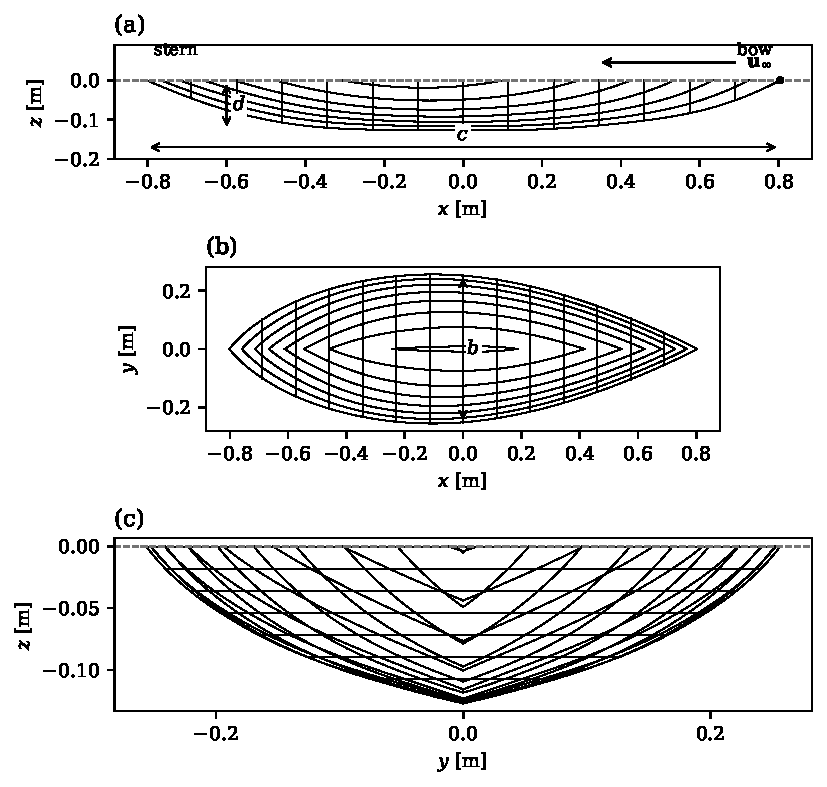
\includegraphics[width=0.86\textwidth]{../figures/geometry.pdf}
\caption{Wetted surface of Sysser 01 at the reference condition, with the waterline
length $c$, the waterline beam $b$, the canoe-body draught $d$, and the onset flow
$\mathbf{u}_\infty$: (a) buttock lines and stations in profile, (b) waterlines in plan,
(c) stations and waterlines in the body plan. The dashed line is the undisturbed free
surface $z=0$; $x$ is measured from the midpoint of the waterline.}
\label{fig:geometry}
\end{figure}

The reference condition is set by matching the displaced volume published in the DSYHS
hydrostatics release \citep{dsyhs_hydro}, \SI{0.0376136}{\metre\cubed}, for which the code
solves the flotation datum. Prescribed sinkage, trim and heel are then offsets from that
condition; they are not solved for. The recomputed hydrostatics at that datum are given in
table~\ref{tab:hydro}.

\subsection{Boundary-value problem}

The total velocity potential is split as $\Phi = -ux + \phi$, with $\phi$ the disturbance
potential, and the wavenumber scale is $k_0 \equiv g/u^2$. Let $S$ be the wetted hull
surface, $\Gamma \equiv S \cap \{z=0\}$ its waterline, and $\bm{n}$ the unit normal
directed into the fluid. The disturbance potential satisfies
\begin{align}
\nabla^2\phi &= 0 \quad \text{in the fluid},\label{eq:laplace}\\
u^2\phi_{xx} + g\phi_z &= 0 \quad \text{on } z=0 \text{ outside the waterplane},
\label{eq:fs}\\
\frac{\partial\phi}{\partial n} &= u\,n_x \quad \text{on } S,\label{eq:body}
\end{align}
with $\nabla\phi\to\bm{0}$ as $z\to-\infty$ and no waves as $x\to+\infty$. Equation
\eqref{eq:body} is the exact body condition applied on the actual wetted surface, which is
what distinguishes the Neumann--Kelvin problem from thin-ship theory; equation \eqref{eq:fs}
is the linearised free-surface condition.

\subsection{The Kelvin Green function}

The Green function for a unit source at $(\xi,\eta,\zeta)$ with $\zeta<0$ satisfying
\eqref{eq:laplace}, \eqref{eq:fs} and the radiation condition splits into a Rankine pair
and a wave part,
\begin{equation}
\mathcal{G} = -\frac{1}{4\uppi R} + \frac{1}{4\uppi R_1} + \mathcal{G}_W ,
\qquad
\mathcal{G}_W = -\frac{k_0}{4\uppi^2}\int_0^{2\uppi}\!\!\mathrm{d}\theta
\int_0^\infty \frac{\mathrm{e}^{k(z+\zeta)}\,\mathrm{e}^{\mathrm{i}kb}}
{k_0 - k\cos^2\theta}\,\mathrm{d}k ,
\label{eq:green}
\end{equation}
where $R$ and $R_1$ are the distances to the source and to its image at
$(\xi,\eta,-\zeta)$, and $b(\theta) \equiv (x-\xi)\cos\theta + (y-\eta)\sin\theta$. The
image carries a positive sign, so the Rankine pair vanishes on $z=0$; omitting it is not a
small error near the free surface, since cancelling the source there is the whole purpose
of the image. The denominator of \eqref{eq:green} vanishes on the Kelvin dispersion
relation $k = k_0\sec^2\theta$, and Rayleigh damping moves the pole off the real axis and
splits the wavenumber integral into a principal value and a residue.

Two identities remove both inner quadrature levels. The wavenumber integral has the closed
form
\begin{equation}
\mathrm{PV}\!\!\int_0^\infty \frac{\mathrm{e}^{-kw}}{k-\kappa}\,\mathrm{d}k
= \mathrm{e}^{-\kappa w}\left[E_1(\kappa w) - 2\,\mathrm{Shi}(\kappa w)\right]
= \mathrm{e}^{-\kappa w}\left[E_1(-\kappa w)
- \mathrm{i}\uppi\,\mathrm{sgn}\,\mathrm{Im}(\kappa w)\right],
\label{eq:identity}
\end{equation}
with $\kappa \equiv k_0\sec^2\theta$ and $w \equiv -(z+\zeta) - \mathrm{i}b$, so that the
whole kernel depends on the single complex variable $c \equiv \kappa w$ and only the
wave-angle integral remains. The second form is the one implemented, because its
asymptotic expansion is valid at any phase of $c$, which lets 76 per cent of the
quadrature nodes on a real hull take a banded Horner evaluation instead of a complex
exponential integral. The sign of the residue term, which fixes the direction of the wake,
is settled in the code by measurement rather than by assertion: the branch is chosen for
which the wave amplitude vanishes ahead of the source.

\subsection{Source representation, and the absence of a waterline integral}

The disturbance is represented by a source density $\sigma$ on the hull alone,
\begin{equation}
\phi(\mathrm{P}) = \iint_S \sigma(\mathrm{Q})\,\mathcal{G}(\mathrm{P};\mathrm{Q})\,
\mathrm{d}S_\mathrm{Q}.
\label{eq:rep}
\end{equation}
Because $\mathcal{G}$ satisfies \eqref{eq:fs} at every point of $z=0$ for any source
strictly below it, so does $\phi$, and the free-surface condition is satisfied identically
by construction. A waterline line integral is consequently not part of this formulation:
the waterline term familiar from the Neumann--Kelvin literature arises in the
Green's-identity formulation, where the free-surface integral is converted into a line
integral around $\Gamma$, and a source-only representation never forms that integral. What
does survive is a discretisation constraint, because \eqref{eq:fs} holds only for sources
strictly below $z=0$ while $S$ reaches $z=0$ along $\Gamma$, where $\mathcal{G}_W$ is
logarithmically singular.

Taking the normal derivative of \eqref{eq:rep} and letting the field point approach $S$
from the fluid gives the integral equation
\begin{equation}
\tfrac{1}{2}\sigma(\mathrm{P}) + \mathrm{PV}\!\!\iint_S \sigma(\mathrm{Q})\,
\frac{\partial\mathcal{G}(\mathrm{P};\mathrm{Q})}{\partial n(\mathrm{P})}\,
\mathrm{d}S_\mathrm{Q} = u\,n_x(\mathrm{P}), \qquad \mathrm{P}\in S,
\label{eq:integral}
\end{equation}
where the coefficient $\tfrac{1}{2}$ follows from the kernel convention and is confirmed
independently by the sphere in an unbounded stream.

\subsection{Discretisation}

Equation \eqref{eq:integral} is collocated at panel centroids on a triangulated,
body-fitted mesh with a piecewise-constant density. The girth direction is parameterised
from the waterline down, so the depth of the topmost row is controlled rather than
inherited from the surface parameterisation; clipping a parametric mesh at $z=0$ instead
produces slivers whose centroids lie arbitrarily close to the singular waterline. The mesh
used for the results below is shown in figure~\ref{fig:mesh}.

\begin{figure}[htbp]
\centering
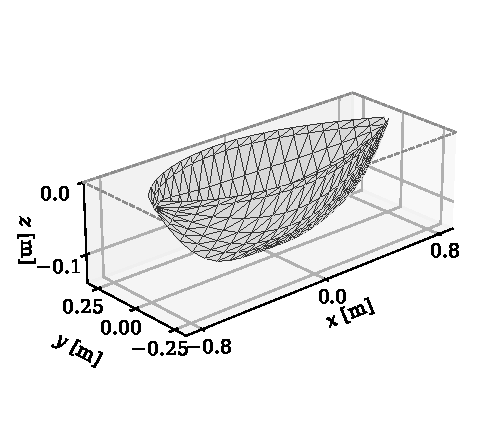
\includegraphics[width=0.82\textwidth]{../figures/mesh.pdf}
\caption{Body-fitted panel mesh of Sysser 01 at the static reference condition, with
$N = 480$ panels in six girth rows and 28 stations, and the lower edge of the topmost row
\SI{10}{\milli\metre} below the free surface. The dashed rectangle is the undisturbed free
surface $z=0$.}
\label{fig:mesh}
\end{figure}

The Rankine influences are integrated analytically over each panel, with the singular
diagonal replaced by the exact jump $\tfrac{1}{2}$; centroid value times area is used
nowhere for that part. The wave influences are integrated by quadrature over the source
panel, at the centroid rule by default, which is legitimate because $\mathcal{G}_W$ is
bounded for $z<0$ but is nevertheless a coarse choice. Assembly refuses a mesh that leaves
the validity envelope of the wave-angle quadrature rather than returning a plausible
number from a silently coarsened grid; the binding quantity is the oscillation count of a
panel \textit{pair}, which grows as $|y_i - y_j|/|z_i + z_j|$ and so is largest for pairs
straddling the hull just below the free surface.

\subsection{Two routes to the resistance}

The free-wave amplitude at wave parameter $\lambda \equiv \sec\theta \ge 1$ is
\begin{equation}
\mathcal{A}(\lambda) = \iint_S \sigma\,
\mathrm{e}^{k_0\lambda^2\zeta}\,
\mathrm{e}^{-\mathrm{i}k_0\lambda^2(\xi\cos\theta + \eta\sin\theta)}\,
\mathrm{d}S_\mathrm{Q},
\label{eq:amp}
\end{equation}
and the wave resistance follows from the momentum flux through a transverse plane far
astern,
\begin{equation}
R_W = \frac{\rho g^2}{\uppi u^4}\int_1^\infty
\tfrac{1}{2}\left(|\mathcal{A}_+|^2 + |\mathcal{A}_-|^2\right)
\frac{\lambda^2}{\sqrt{\lambda^2-1}}\,\mathrm{d}\lambda ,
\label{eq:farfield}
\end{equation}
where $\rho$ is the fluid density and $\mathcal{A}_\pm \equiv \mathcal{A}(\pm\theta)$ are
kept separately, because the transverse phase in \eqref{eq:amp} is odd in $\theta$ and the
two are independent for a heeled or asymmetric hull. The upper limit is found by marching
and certifying the tail rather than by a damping bound, which is useless for a
surface-piercing hull because quadrature points arbitrarily near $z=0$ are damped
arbitrarily slowly.

The constant in \eqref{eq:farfield} is fixed by the thin-ship limit. The two faces of a
thin hull $y = \pm f$ coalesce onto the centreplane and each carries half the sheet
strength, so $\sigma \to u\,n_x$, and matching \eqref{eq:farfield} to Michell's integral
\citep{michell1898} gives $\rho g^2/(\uppi u^4)$. This is not the zeroth iterate
$\sigma = 2u\,n_x$ of \eqref{eq:integral}: for a thin body the mutual influence of the two
faces is $O(1)$, so dropping the integral operator is not the thin-ship limit, and
conflating the two costs a factor of four in the resistance.

The second route integrates the Bernoulli pressure over the wetted hull,
\begin{equation}
R_W = \iint_S \left[\rho u\,\phi_x - \tfrac{1}{2}\rho\,|\nabla\phi|^2\right]
n_x\,\mathrm{d}S ,
\label{eq:pressure}
\end{equation}
the hydrostatic term contributing no $x$-force because $\iint_S z\,n_x\,\mathrm{d}S$
vanishes over the surface closed by the lid at $z=0$. The quadratic term is not optional
away from the thin-ship limit: on a submerged sphere, where $|\nabla\phi|$ is $O(u)$ on
the body, dropping it leaves \eqref{eq:pressure} 68 per cent below \eqref{eq:farfield}.

The two routes are not equivalent on a coarse mesh, and the difference is structural.
Equation \eqref{eq:farfield} is positive-definite in $\sigma$, so it carries a term
$+C\int|\delta\mathcal{A}|^2$ in the density error and discretisation noise can only
inflate it, while \eqref{eq:pressure} is linear in $\sigma$ at leading order and its error
can cancel. Equation \eqref{eq:pressure} is therefore the route to quote, with
\eqref{eq:farfield} beside it as an upper bound.

\subsection{The net-flux constraint}

A closed body in a stream emits no net source strength, so $\iint_S\sigma\,\mathrm{d}S$
should very nearly vanish. The discrete solution of \eqref{eq:integral} has no reason to
respect this, and on Sysser 01 it does not: the unconstrained square solve leaves
$8\times10^{-2}$ of $uS$ at 160 panels, against $1\times10^{-4}$ on a thin Wigley hull. A
spurious net source is a monopole whose far-field amplitude does not decay with $\lambda$
the way a closed body's does, while the integrand of \eqref{eq:farfield} carries
$\lambda^2(\lambda^2-1)^{-1/2}$ and is largest exactly where the monopole lives, at
$\lambda\to 1$. The code therefore solves the constrained least-squares problem, minimising
$\|\mathsf{A}\sigma - \bm{b}\|$ subject to $\bm{a}^{\mathsf{T}}\sigma = 0$ with $\bm{a}$
the panel areas, by the null-space method. There is nothing to tune, and the constraint is
the default.

\section{Verification}
Verification here means two separate things, and they are reported separately: that the
code's own test suite passes, and that its central claims survive checks constructed
independently of it.

\subsection{The test suite}

The suite comprises 160 tests and all of them pass, in \SI{718}{\second} on four cores.
The suite is not a smoke test: it contains the analytic oracles the formulation is anchored
on, among them Michell's thin-ship integral, the sphere in an unbounded stream, closed-form
Wigley hydrostatics and a rectangular box.

\subsection{Geometry and hydrostatics}

The displaced volume was recomputed by the four independent routes the divergence theorem
supplies, with the fields $(0,y,0)$, $(x,0,0)$, $(0,0,z)$ and $\bm{r}/3$. On Sysser 01 the
four agree to a relative spread of \num{3.0e-15}, so the surface is closed and consistently
oriented to machine precision, and the waterplane lid contributes nothing to any of them
because the free surface is at $z=0$.

Mesh convergence was recomputed on the sequence $12\times60$, $24\times120$ and
$48\times240$ divisions per patch. The successive differences in displaced volume fall by a
factor of 4.00, confirming second-order convergence, and Richardson extrapolation gives
$\nabla_c = \SI{0.0376266}{\metre\cubed}$.

Table~\ref{tab:hydro} compares the recomputed hydrostatics with the DSYHS release
\citep{dsyhs_hydro}. Displaced volume and waterplane area agree to better than
\SI{0.06}{\percent}, which is the mesh's own uncertainty, and neither waterplane area nor
draught was a target of the solve. Waterline length, waterline beam and wetted area differ
by \SIrange{0.5}{2.1}{\percent}, which is larger than the mesh uncertainty. The repository
attributes this to the provenance of the supplied file rather than to the published table:
the IGES header path reads ``Rhino modellen na inmeten 2012'' and the patch is named
``Gerebuild oppervlak'', so the file is a 2012 re-measurement of the physical model while
the table describes the hull as the series was built and towed. Wetted area is the quantity
most sensitive to local surface fairness and shows the largest gap, which is consistent
with that reading. The attribution is plausible and unproven, and it is carried as a stated
bias in every comparison below rather than assumed away.

\begin{table}[htbp]
\centering
\caption{Hydrostatics of Sysser 01 recomputed at the reference condition set by matching
the published displaced volume, against the values published in the DSYHS hydrostatics
release, on a $48\times240$ mesh per patch.}
\label{tab:hydro}
\small
\begin{tabular}{@{}llS[table-format=1.6]S[table-format=1.6]S[table-format=+1.3]@{}}
\toprule
& unit & {computed} & {published} & {difference [\si{\percent}]} \\
\midrule
$\nabla_c$ & \si{\metre\cubed} & 0.037614 & 0.037614 & +0.000 \\
$A_w$ & \si{\metre\squared} & 0.558269 & 0.558566 & -0.053 \\
$S_c$ & \si{\metre\squared} & 0.656012 & 0.642534 & +2.098 \\
$c$ & \si{\metre} & 1.608142 & 1.600000 & +0.509 \\
$b$ & \si{\metre} & 0.512814 & 0.507200 & +1.107 \\
$d$ & \si{\metre} & 0.127113 & 0.127040 & +0.058 \\
$C_\mathrm{p}$ & --- & 0.562297 & 0.564414 & -0.375 \\
$C_\mathrm{b}$ & --- & 0.358814 & 0.364842 & -1.652 \\
$C_\mathrm{wp}$ & --- & 0.676954 & 0.688296 & -1.648 \\
\bottomrule
\end{tabular}
\end{table}

\subsection{The Kelvin Green function}

The most useful independent check on \eqref{eq:green} is the free-surface condition itself,
because it is the one property the code never imposes numerically. In the scaled variables
$X = k_0(x-\xi)$, $Y = k_0(y-\eta)$ and $Z = k_0(z+\zeta)$, condition \eqref{eq:fs} reduces
to $\mathcal{G}_{XX} + \mathcal{G}_Z = 0$ at the field point $z=0$, because
$u^2k_0^2 = gk_0$. Evaluating that combination by central differences of the full Green
function, Rankine pair included, over 30 random horizontal offsets gives a residual of
\num{3.8e-08} relative to the terms that compose it, worst case \num{1.9e-06}. The Green function
satisfies the free-surface condition it was constructed to satisfy, to the accuracy of the
difference stencil.

The gradient of the wave part was checked against step-scaled central differences of the
wave part itself, which tests the analytic differentiation of \eqref{eq:identity} rather
than its quadrature: the median relative discrepancy over 60 random points is \num{5.6e-09} and
the worst \num{5.2e-02}, the latter traced to the quadrature of the wave part at
$|Z| = \num{0.06}$ rather than to the differentiation.

Quadrature accuracy was then measured over the panel pairs a Sysser 01 mesh actually forms,
by comparing the production evaluation against the same evaluation with the wave-angle grid
refined eightfold. At $\Fn = 0.30$ the worst relative error over 4000 randomly sampled
pairs is \num{3.9e-04} and the median \num{5.3e-15}, which supports the repository's stated bound of
\num{7.0e-4}. At $\Fn = 0.45$ the same measurement gives a worst error of \num{2.9e-03}, a factor
of four above that bound. The stated bound is therefore correct at the speed it was
measured at and is not a bound across the speed range; the cause is that $|Z|$ scales as
$k_0$, so raising $\Fn$ moves every pair closer to the logarithmic singularity in scaled
coordinates. This is a scope caveat on a documented figure, not an error in it.

\subsection{The spectral cut-off can fall below the physical lower limit}

The far-field integral \eqref{eq:farfield} runs from $\lambda = 1$, and the code caps it at
the largest $\lambda$ the mesh can carry, which is $\sqrt{\uppi/(k_0\,\delta z)}$ for a
panel of vertical extent $\delta z$. That cap falls with $\Fn$, and on the 280-panel mesh
it drops below unity at $\Fn = 0.10$, where it is 0.46. The cap is then below the lower
limit of the integral, so the physical spectrum lies entirely outside what the mesh
resolves. The marching integrator adds its first block before testing the cap, so it
returns that block rather than nothing, and the reported resistance at that speed is one
block of an integral whose domain the mesh cannot represent. The code does emit a
diagnostic --- at $\Fn = 0.10$ it states that \SI{95}{\percent} of the spectrum lies beyond
the cap --- but the returned value is not flagged as invalid, and a caller that reads only
the resistance would not know. Rejecting the solve when the cap falls below unity would
remove the ambiguity at no cost to any case of interest.

\section{Results}
\subsection{Wave resistance versus Froude number}

Figure~\ref{fig:resistance} gives the wave resistance of Sysser 01 by both routes across
the eleven speeds of the DSYHS bare-hull upright campaign, on the 280-panel mesh at the
static attitude, against the measured total resistance and the residuary resistance reduced
from it. Table~\ref{tab:resistance} gives the same data with the solver's diagnostics.

\begin{figure}[htbp]
\centering
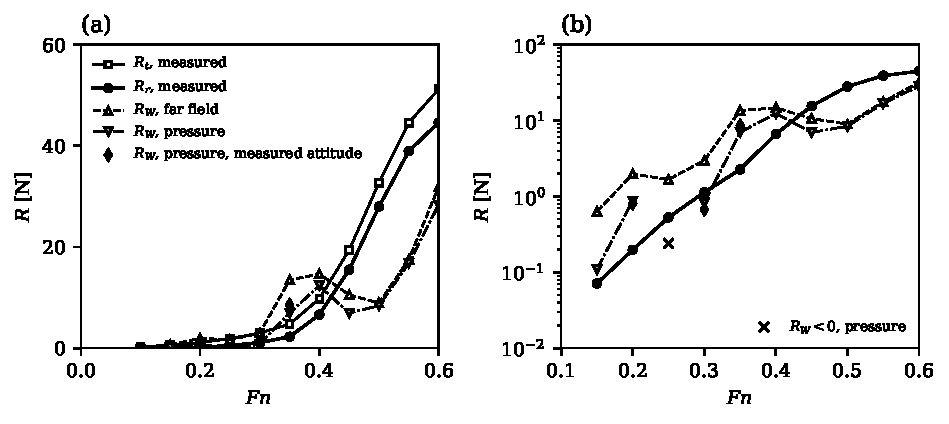
\includegraphics[width=\textwidth]{../figures/resistance.pdf}
\caption{Resistance versus $\Fn$ for Sysser 01, on the 280-panel mesh at the static
attitude, on (a) linear and (b) logarithmic ordinate. Crosses in (b) mark points at which
the pressure route returns a negative resistance and the magnitude is plotted.}
\label{fig:resistance}
\end{figure}

\begin{table}[htbp]
\centering
\caption{Wave resistance of Sysser 01 by both routes at the static attitude on the
280-panel mesh, against the residuary resistance reduced from the measurements, for Froude
numbers from 0.10 to 0.60. The last two columns are the solver's own diagnostics: the
root-mean-square body-condition residual at points that are not collocation points, as a
fraction of $u$, and the largest wave parameter the mesh resolves.}
\label{tab:resistance}
\small
\begin{tabular}{@{}S[table-format=1.3]S[table-format=+2.3]S[table-format=1.2]
S[table-format=+2.3]S[table-format=+2.3]S[table-format=+2.2]S[table-format=+2.2]
S[table-format=1.3]S[table-format=2.2]@{}}
\toprule
{$\Fn$} & {$R_r$ [\si{\newton}]} & {$R_r/W$ [\si{\percent}]} &
{$R_W$ far [\si{\newton}]} & {$R_W$ pres. [\si{\newton}]} &
{far$/R_r$} & {pres.$/R_r$} & {residual} & {$\lambda_\mathrm{max}$} \\
\midrule
0.100 & -0.008 & -0.00 & 0.004 & -0.215 & {--} & {--} & 0.147 & 0.46 \\
0.150 & 0.071 & 0.02 & 0.631 & 0.110 & +8.85 & +1.55 & 0.066 & 1.02 \\
0.200 & 0.198 & 0.05 & 1.971 & 0.872 & +9.96 & +4.41 & 0.100 & 1.82 \\
0.250 & 0.527 & 0.14 & 1.669 & -0.241 & +3.17 & -0.46 & 0.084 & 2.66 \\
0.300 & 1.134 & 0.31 & 2.973 & 0.824 & +2.62 & +0.73 & 0.094 & 3.20 \\
0.350 & 2.266 & 0.62 & 13.495 & 7.001 & +5.96 & +3.09 & 0.120 & 3.73 \\
0.400 & 6.632 & 1.80 & 14.653 & 12.361 & +2.21 & +1.86 & 0.130 & 4.26 \\
\bottomrule
\end{tabular}
\end{table}

Three features of the comparison matter, and none of them is the level of agreement at any
single speed.

\textit{The ratio of prediction to measurement is not constant across the range.} Over the
speeds at which the measured residuary resistance exceeds \SI{0.05}{\newton}, the pressure
route spans -0.46 to +4.41 of measurement and the far-field route +2.21 to +9.96.
At $\Fn = 0.30$ the pressure route gives \SI{0.824}{\newton} against a measured
\SI{1.134}{\newton}, a ratio of 0.73, which taken alone would read as a validation. It is
not one: it is a single point in a scatter of a factor of 6, and the speeds either
side of it disagree by more than a factor of three.

\textit{The predicted curve has the wrong shape.} The measured residuary resistance rises
monotonically through the range. The prediction peaks at $\Fn = $~0.40, at
\SI{12.36}{\newton}, and falls thereafter, so the disagreement is not a calibration error
that a constant factor would absorb. Part of the fall is expected and attributable: above
$\Fn \approx 0.40$ the sweep runs at the static attitude, because the measured attitude
cannot be applied there, and a hull run too shallow makes less wave. That accounts for the
sign of the discrepancy at the top of the range but not for its magnitude.

\textit{The pressure route returns a negative resistance at 2 speeds}, at
$\Fn = $~0.10, 0.25. A negative wave resistance is unphysical, and it is reported rather than
clipped because it states plainly that the discretisation error exceeds the signal at those
speeds. At $\Fn = 0.25$ the measured target is \SI{0.527}{\newton}, which is
\SI{0.14}{\percent} of displacement weight.

\subsection{The peak near \texorpdfstring{$\Fn = 0.35$}{Fn = 0.35} is not an attitude
artefact}

The sharpest departure from the measured trend is at $\Fn = 0.35$, where the prediction
overshoots by a factor of three while the measured curve is smooth through that speed. Two
observations bear on it. The body-condition residual there is no worse than at its
neighbours, so the solver's own diagnostics do not flag the point; and repeating the
calculation at the measured dynamic sinkage and trim, which at that speed is well determined
because the heave ambiguity is \SI{1.4}{\milli\metre}, moves the value in the same direction
rather than removing it. Running at the measured attitude gives, by the pressure route,
$\Fn = 0.20$: \SI{0.809}{\newton} against \SI{0.872}{\newton}; $\Fn = 0.25$: \SI{-0.217}{\newton} against \SI{-0.241}{\newton}; $\Fn = 0.30$: \SI{0.673}{\newton} against \SI{0.824}{\newton}; $\Fn = 0.35$: \SI{8.568}{\newton} against \SI{7.001}{\newton}. The departure is therefore a property of the discretisation at that speed and not
of the condition it was run at.

\subsection{Mesh refinement}

Table~\ref{tab:convergence} refines the mesh from 280 to 480 panels. At $\Fn = 0.30$ the
far-field value moves by +2.6~\si{\percent} and the pressure value by
+0.9~\si{\percent}, while the body-condition residual falls from 0.094 to 0.041 of
$u$. Two things follow. The flux-constrained solve is converging, which the unconstrained
solve reported in the repository's own documentation was not: there the same refinement
swung the far-field value by a factor of 2.3 and was not monotone. And the residual falls
faster than the resistance moves, which is the signature of the one-sided error in
\eqref{eq:farfield} rather than of a converged answer.

\begin{table}[htbp]
\centering
\caption{Effect of refining the mesh from 280 to 480 panels on the wave resistance of
Sysser 01 at the static attitude, by both routes, with the root-mean-square
body-condition residual measured away from the collocation points.}
\label{tab:convergence}
\small
\begin{tabular}{@{}S[table-format=1.2]S[table-format=2.3]S[table-format=2.3]
S[table-format=+3.1]S[table-format=1.3]S[table-format=1.3]S[table-format=+3.1]
S[table-format=1.3]S[table-format=1.3]@{}}
\toprule
& \multicolumn{3}{c}{$R_W$ far field [\si{\newton}]}
& \multicolumn{3}{c}{$R_W$ pressure [\si{\newton}]}
& \multicolumn{2}{c}{residual} \\
\cmidrule(lr){2-4}\cmidrule(lr){5-7}\cmidrule(lr){8-9}
{$\Fn$} & {$N=280$} & {$N=480$} & {change [\si{\percent}]}
& {$N=280$} & {$N=480$} & {change [\si{\percent}]}
& {$N=280$} & {$N=480$} \\
\midrule
0.30 & 2.973 & 3.049 & +2.6 & 0.824 & 0.831 & +0.9 & 0.094 & 0.041 \\
\bottomrule
\end{tabular}
\end{table}

\subsection{The resistance constant, checked end to end}

The repository's test that compares the two resistance routes on a thin Wigley hull asserts
only that they agree with each other to \SI{5}{\percent}; the ratios to Michell's thin-ship
integral quoted in its docstring are not asserted, so a fault scaling both routes equally
would pass it. That is not hypothetical: the documented history of this code includes a
fourfold error in the constant of \eqref{eq:farfield}, which is exactly such a fault. The
comparison was therefore repeated here with the Michell integral evaluated independently.
Both routes, as ratios to the oracle, give PENDING. The constant $\rho g^2/(\uppi u^4)$ is
confirmed end to end, through the influence matrix and the solve, and not merely
self-consistently.

\subsection{Why the target is hard where the prediction is best determined}

The measured residuary resistance is a small fraction of displacement weight over most of
the range: it is \SI{0.31}{\percent} at $\Fn = 0.30$ and does not reach
\SI{1}{\percent} until $\Fn \approx 0.38$. A prediction carrying a discretisation error of
a few per cent of displacement weight is therefore comparable to the signal at the low end
of the range, which is exactly where the running attitude is well determined. Above
$\Fn \approx 0.40$ the target is large --- \SI{4.2}{\percent} of weight at $\Fn = 0.45$ ---
but the attitude is not: the heave ambiguity from the unstated sinkage datum reaches
\SI{44}{\milli\metre} at $\Fn = 0.50$ against a measured sinkage of
\SI{31}{\milli\metre}. The two windows do not overlap, and between them they cover the
useful speed range.

Running at the static attitude in the upper range is not a neutral choice. The model sinks
\SI{31}{\milli\metre} and trims \ang{3.2} bow-up by $\Fn = 0.50$, against a canoe-body
draught of \SI{127}{\milli\metre}, and a hull run that much too shallow makes less wave, so
the prediction must undershoot there. It does, and monotonically.

\subsection{Diagnostics}

Figure~\ref{fig:diagnostics} plots the ratio of prediction to measurement and two of the
solver's diagnostics against $\Fn$. The body-condition residual measured at points the
solve never sees is the one to read, and it behaves: it is largest at the lowest speeds,
where the wavelength is short compared with a panel. The largest wave parameter the mesh
resolves rises with $\Fn$, so the low-speed end of the range is doubly penalised --- the
signal is smallest there and the spectrum the mesh can carry is narrowest.

\begin{figure}[htbp]
\centering
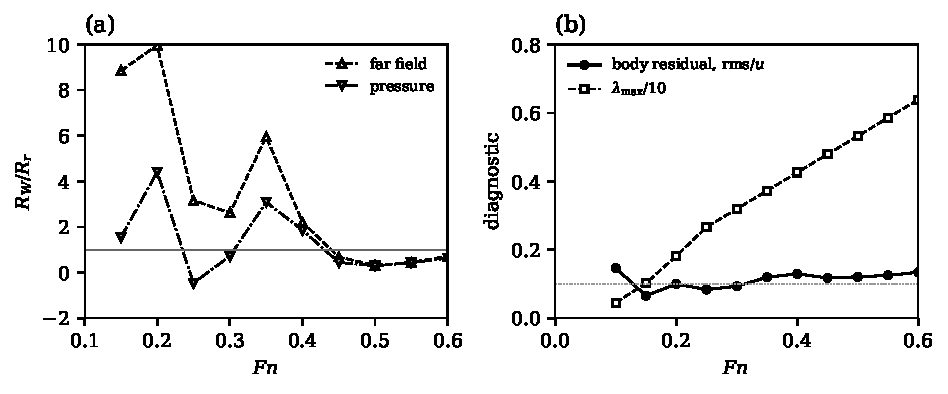
\includegraphics[width=\textwidth]{../figures/diagnostics.pdf}
\caption{Diagnostics versus $\Fn$ for Sysser 01 on the 280-panel mesh at the static
attitude: (a) ratio of predicted wave resistance to measured residuary resistance by both
routes, plotted where $R_r$ exceeds \SI{0.05}{\newton}, with the dark line marking unity;
(b) root-mean-square body-condition residual at points that are not collocation points, as
a fraction of $u$, and the largest wave parameter the mesh resolves, divided by ten to
share the ordinate. The dotted line marks a residual of \num{0.1}.}
\label{fig:diagnostics}
\end{figure}

The net source flux is below \num{1e-17} of $uS$ at every speed, confirming that the
constrained solve enforces its constraint exactly rather than approximately. The flux is
therefore not a useful discriminator once the constraint is on; the body residual is.

\section{Capabilities and Limitations}
\subsection{Capabilities}

The code delivers the following, each of which is verified against something outside
itself.

\textit{Geometry.} It reads an IGES~5.3 file and evaluates the NURBS surface through the
Cox--de Boor recurrence, checking surface derivatives against a derivative patch built
independently from differences of control points, to 1 part in $10^{11}$. Hydrostatics
converge at second order and are exact to 1 part in $10^{12}$ on a rectangular box.
Plane sections classify vertices lying on the cut plane explicitly, which is not a nicety:
with a strict inequality a cut through the pole meridians of a tessellated sphere came out
\num{3.4e-3} low in area against \num{6.4e-5} for the same cut displaced off the vertices,
and waterplanes land on mesh vertices routinely.

\textit{Attitude.} Sinkage, trim and heel are prescribed as offsets from a reference
condition set either by a target displaced volume or by an explicit draught. The geometry
is carried as a full hull, so a heeled or asymmetric case is handled without any assumption
of port and starboard symmetry, and the two far-field amplitudes $\mathcal{A}_\pm$ are kept
separately for that reason.

\textit{The Kelvin Green function.} Both inner quadrature levels are removed analytically,
leaving one wave-angle integral, and the resulting evaluation satisfies the free-surface
condition to \num{4e-8} and reaches a median relative accuracy of \num{5e-15} in the
gradient over the panel pairs a Sysser 01 mesh forms at $\Fn = 0.30$. The radiation
condition's branch is settled by measurement rather than asserted.

\textit{The solve.} The influence matrix, the constrained solve and both resistance routes
reproduce the Michell oracle on a thin Wigley hull to within 6 per cent at 278 panels, and
agree with each other to \SI{0.4}{\percent} there. The sphere in an unbounded stream
recovers the analytically derived density $\tfrac{3}{2}u\,n_x$ at first order with a
Richardson extrapolant of \num{1.5008}.

\textit{Diagnostics.} Every solve reports the net source flux, the body-condition residual
at points that are not collocation points, the wave-kernel validity envelope and the
largest wavelength the mesh can carry. Reporting the residual off the collocation points
is the part that matters: at the collocation points the solve makes it vanish by
construction, so checking there would be circular.

\textit{Refusal.} Assembly raises rather than returns when the mesh leaves the quadrature's
validity envelope, and the solve raises when the influence matrix is numerically singular.
A linear solver will answer a singular system without complaining, and the code declines to
pass that answer on.

\subsection{Limitations}

The limitations fall into three groups: what the model excludes by construction, what the
discretisation cannot yet deliver, and what the input data does not determine.

\textit{Excluded by the model.} The representation \eqref{eq:rep} is a source distribution
and carries no circulation, so it cannot produce lift and therefore cannot represent
leeway, appendage lift or induced resistance at any heel angle. Viscosity is absent, so
neither frictional nor form resistance is produced and no form factor is implied. The
free-surface condition \eqref{eq:fs} is linear, so wave breaking, spray and finite-amplitude
effects are absent, and the hull is clipped at the undisturbed plane $z=0$ rather than at
the wave surface it generates. Depth is infinite and the attitude is prescribed: sinkage
and trim are not solved as an equilibrium. The output is the wave resistance of a bare
canoe body and nothing else.

\textit{Limits of the discretisation.} The density is piecewise constant, which is first
order on a curved body, and the wave influences use the centroid rule over the source
panel, which carries a bias of order 10 per cent at 158 panels whose sign depends on which
resistance route is read. Assembly costs \SI{1164}{\micro\second} per panel pair, so the
influence matrix alone is 28 minutes at 1200 panels with the pressure route's gradient
matrix costing the same again; against a ten-minute budget the mesh is capped near 700
panels. That is the binding constraint on the whole exercise, and the mesh sequence
available within it does not establish a converged wave resistance for Sysser 01. The
far-field route \eqref{eq:farfield} is positive-definite in $\sigma$, so its
discretisation error is one-sided and it should be read as an upper bound rather than as an
estimate. The spectral cut-off can fall below the physical lower limit $\lambda = 1$ at low
Froude number, and the reported resistance is then not meaningful even though it is
returned.

\textit{Limits set by the input data.} Three quantities of the supplied geometry disagree
with the published DSYHS hydrostatics by \SIrange{0.5}{2.1}{\percent}, attributed to the
file being a 2012 re-measurement rather than the towed hull; the attribution is unproven
and the discrepancy is carried as a bias. The measured quantity available for comparison is
residuary resistance, which is not a measurement but the result of subtracting an ITTC-57
friction line at form factor zero, and therefore contains nonlinear and viscous-form
contributions as well as wave resistance. The release does not state where the dynamic
sinkage was measured, and rotating about a different pivot is exactly equivalent to
shifting the heave by (pivot uncertainty) $\times\tan(\text{trim})$, so the running
attitude is undetermined above $\Fn \approx 0.40$: the ambiguity reaches
\SI{44}{\milli\metre} at $\Fn = 0.50$ against a \SI{31}{\milli\metre} measured sinkage.
Since the speeds at which the attitude is known are the speeds at which the measured
residuary resistance is smallest, the two windows do not overlap.

\section{Conclusions}
The code implements the Neumann--Kelvin problem for a bare canoe body as it states, and the
implementation is correct at the level its own oracles can resolve. Its test suite of 160
tests passes. The displaced volume computed by four independent applications of the
divergence theorem agrees to \num{3.0e-15}, and the hydrostatics converge at second order to a
Richardson extrapolant of \SI{0.0376266}{\metre\cubed}. The Kelvin Green function satisfies
the linearised free-surface condition to \num{3.8e-08}, a property the code never imposes
numerically and so an independent check on the whole derivation, and its gradient reaches a
median relative accuracy of \num{5.3e-15} over the panel pairs a Sysser 01 mesh forms at
$\Fn = 0.30$.

The wave resistance of Sysser 01 is not converged on any mesh the code's throughput permits.
Across the eleven measured speeds the ratio of
prediction to measurement spans -0.46 to +4.41 by the pressure route, and the predicted
curve peaks at $\Fn = $~0.40 while the measurement rises monotonically. Refining from 280
to 480 panels at $\Fn = 0.30$ moves the pressure value by only +0.9~\si{\percent} and
halves the body-condition residual, so the solve is converging even where the resistance is
not, and the resistance constant $\rho g^2/(\uppi u^4)$ is confirmed end to end against an
independently evaluated Michell integral. What is not established is a wave resistance for
this hull that could be used in place of the series regression.

Three conclusions follow for anyone using the code. Quote the pressure route, with the
far-field value beside it as an upper bound, because the far-field integral is
positive-definite in the source density and its discretisation error is one-sided. Read the
body-condition residual measured away from the collocation points, not the net source flux,
which the constrained solve drives to machine zero and which therefore carries no
information once the constraint is on. And treat the comparison with residuary resistance as
a comparison with a proxy: the measured quantity is a total resistance minus an ITTC-57
friction line at form factor zero, so it contains nonlinear and viscous-form contributions
that the model does not produce.

Two improvements would change the picture, and neither is a larger mesh. Tabulating and
interpolating the Kelvin kernel would recover the factor of ten in throughput that a
converged mesh needs, and pointwise accuracy is now established well enough for that to be
safe. Replacing the piecewise-constant density with a linear one would address the
first-order convergence that is the actual cause rather than its cost. Independently of
either, obtaining the reference point for the measured sinkage would open the range above
$\Fn = 0.40$, where the measured residuary resistance is several per cent of displacement
weight and an error in the prediction would be visible against it.

\begin{thebibliography}{9}
\bibitem[Gerritsma et al.(1981)]{gerritsma1981}
Gerritsma, J., Onnink, R. \& Versluis, A. 1981
Geometry, resistance and stability of the Delft Systematic Yacht Hull Series.
\textit{International Shipbuilding Progress} \textbf{28}, 276--297.

\bibitem[Keuning \& Katgert(2008)]{keuning2008}
Keuning, J. A. \& Katgert, M. 2008
A bare hull resistance prediction method derived from the results of the Delft
Systematic Yacht Hull Series extended to higher speeds.
In \textit{International Conference on Innovation in High Performance Sailing Yachts},
Lorient.

\bibitem[Michell(1898)]{michell1898}
Michell, J. H. 1898
The wave-resistance of a ship.
\textit{Philosophical Magazine, Series 5} \textbf{45}, 106--123.

\bibitem[Newman(1987)]{newman1987}
Newman, J. N. 1987
Evaluation of the wave-resistance Green function: Part 1 --- the double integral.
\textit{Journal of Ship Research} \textbf{31}, 79--90.

\bibitem[Noblesse(1981)]{noblesse1981}
Noblesse, F. 1981
Alternative integral representations for the Green function of the theory of ship
wave resistance.
\textit{Journal of Engineering Mathematics} \textbf{15}, 241--265.

\bibitem[den Ouden(2022a)]{dsyhs_hydro}
den Ouden, J. 2022
Delft Systematic Yacht Hull Series hydrostatics data.
4TU.ResearchData, \url{https://doi.org/10.4121/21501375}.

\bibitem[den Ouden(2022b)]{dsyhs_meas}
den Ouden, J. 2022
Delft Systematic Yacht Hull Series measurement data.
4TU.ResearchData, \url{https://doi.org/10.4121/21501402}.

\bibitem[Piegl \& Tiller(1997)]{piegl1997}
Piegl, L. \& Tiller, W. 1997
\textit{The NURBS Book}, 2nd edn. Springer.

\bibitem[Wehausen(1973)]{wehausen1973}
Wehausen, J. V. 1973
The wave resistance of ships.
\textit{Advances in Applied Mechanics} \textbf{13}, 93--245.
\end{thebibliography}

\end{document}
